\chapter{Assignment: \protect\\ Clustering vs. Classification}
\label{hw:clustering-classification}

\newthought{Clustering and classification are fundamentally different tasks.} The former tries to find similar data instances and puts them into groups or clusters. The latter looks for the patterns in the data and infers correlations between the features and the target variable. Clustering is a part of unsupervised learning and doesn't require a target variable. Classification is a part of supervised learning and requires a target variable. A target variable is the thing we want to predict. With clustering, we are not predicting anything, but trying to find groups of similar data instances.

\begin{figure}[h]
  \centering
  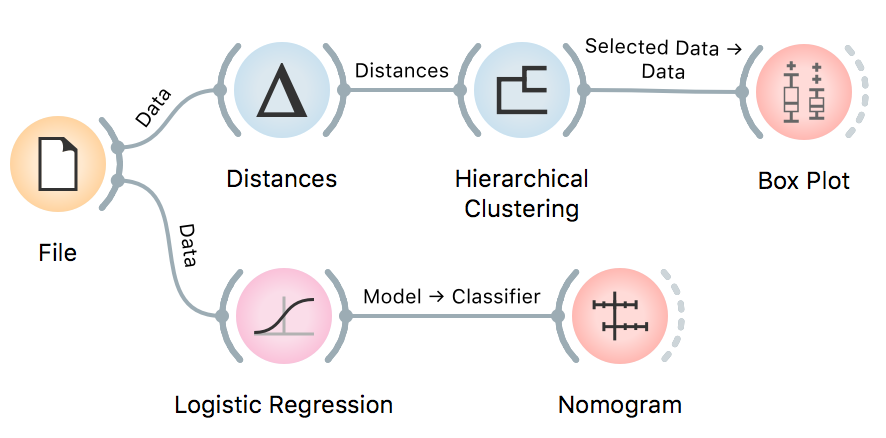
\includegraphics[scale=0.7]{workflow.png}%
  \caption{$\;$}
  \label{fig:wf1}
\end{figure}

For this task, use \textit{heart-disease} data and build a simple hierarchical clustering workflow (with Euclidean distance and Ward linkage) and a logistic regression model and inspect it in a nomogram. In clustering, cut at two clusters. Refer to the workflow above and answer the following questions:

\begin{enumerate}
    \item Explore the groups with \widget{Box Plot}. What is the characteristic of cluster 1 (C1)? What is the characteristic of cluster 2 (C2)?
    \item Which are the top three attributes distinguishing between clusters? Write them down.
    \item In \widget{Nomogram}, which are the three most important attributes for the model?
    \item Are the attributes from clustering the same as those from logistic regression? Why (not)?
    \item \textit{Major vessels colored} is the most important attribute for logistic regression. How well does it split between the clusters?
\end{enumerate}
